\documentclass{article}
\usepackage[english]{babel}
\usepackage[utf8]{inputenc}
\usepackage{fancyhdr}
\usepackage[margin=1in]{geometry}
\usepackage{mathtools}
\usepackage{amssymb}
\usepackage{bm}
\usepackage{amsthm}
\usepackage{centernot}
\usepackage{blindtext}
\usepackage{natbib}
\usepackage{graphicx}
\usepackage{centernot}
\usepackage{pgfplots}
\usepackage{rotating}
\usepackage{mathrsfs}
\def\upint{\mathchoice%
	{\mkern13mu\overline{\vphantom{\intop}\mkern7mu}\mkern-20mu}%
	{\mkern7mu\overline{\vphantom{\intop}\mkern7mu}\mkern-14mu}%
	{\mkern7mu\overline{\vphantom{\intop}\mkern7mu}\mkern-14mu}%
	{\mkern7mu\overline{\vphantom{\intop}\mkern7mu}\mkern-14mu}%
	\int}
\def\lowint{\mkern3mu\underline{\vphantom{\intop}\mkern7mu}\mkern-10mu\int}

\usepackage{hyperref}
\hypersetup{
	colorlinks,
	linkcolor={red!80!black},
	citecolor={blue!80!black},
	urlcolor={blue!80!black}
}
\usepackage[nameinlink,capitalize]{cleveref}

\usepackage[titles]{tocloft}
\renewcommand{\thepart}{\Roman{part} }

\usepackage{tikz}
\newcommand{\N}{\mathbb{N}}
\newcommand{\R}{\mathbb{R}}
\newcommand{\Q}{\mathbb{Q}}
\newcommand{\x}{\mathbf{x}}
\newcommand{\F}{\mathbf{F}}
\newcommand{\f}{\mathbf{f}}
\newcommand{\y}{\mathbf{y}}
\renewcommand{\b}{\mathbf{b}}
\renewcommand{\c}{\mathbf{c}}
\renewcommand{\a}{\mathbf{a}}
\newcommand{\T}{\mathcal{T}}
\newcommand{\h}{\mathbf{h}}
\newcommand{\g}{\mathbf{g}}
\newcommand{\z}{\mathbf{z}}
\newcommand{\ze}{\mathbf{0}}
\newcommand{\Z}{\mathbb{Z}}
\newcommand{\M}{\mathcal{M}}
\newcommand{\norm}[1]{\left\lVert#1\right\rVert}
\newcommand{\abs}[1]{\left\lvert#1\right\rvert}
\newcommand{\brk}[1]{ \left(#1\right] }
\newcommand{\brc}[1]{ \left\{#1\right\} }
\newcommand{\paren}[1]{ \left(#1\right) }
\newcommand{\normop}[1]{\left\lVert#1\right\rVert_\text{op}}
\newcommand{\LL}{\mathcal{L}}
\newcommand{\uni}{\overset{\text{uni}}{\to}}
\DeclareMathOperator{\diam}{diam}
\newcommand{\Prr}[1]{\text{Pr}\left(#1\right)}
\pgfplotsset{my style/.append style={axis x line=middle, axis y line=
		middle, xlabel={$x$}, ylabel={$y$}, axis equal }}

\setcounter{section}{-1}
\theoremstyle{definition}
\newtheorem{proposition}{Proposition}[section]
\newtheorem{theorem}{Theorem}[section]
\newtheorem{lemma}{Lemma}[section]
\newtheorem{definition}{Definition}[section]
\newtheorem{corollary}{Corollary}[section]
\newtheorem{ex}{Exercise}[section]
\newtheorem{note}{Notation}[section]
\newtheorem{example}{Example}[section]
\newtheorem{remark}{Remark}[section]

\renewcommand{\baselinestretch}{1.25} 


\title{Real Analysis}
\author{Noah Jussila}
\date{\today}

\begin{document}
	\maketitle
	\bibliographystyle{chicago}
	\tableofcontents
	
	\section{Introduction}
	This collection of notes is an ongoing project that aims to combine four semesters of real analysis notes into one document. My goal in doing so is to not only stave off the boredom resulting from quarantining due to Covid-19, but also pick and choose from different presentations of standard material in real analysis. 
	\subsection{Prerequisites}
	These notes will assume familiarity with differential and integral calculus, linear algebra, multivariable calculus, basic set theory, and properties of functions (image, preimage, injectivity, etc.) At times, some material, particularly concepts in linear algebra, will be reviewed. Two very good video series that serve as reviews for calculus and linear algebra can be found at this amazing \href{https://www.youtube.com/channel/UCYO_jab_esuFRV4b17AJtAw}{YouTube channel}.
	
	I also will assume familiarity with basic styles of proof (contradiction, contrapositive, etc.). I will try \textit{very hard} to be as detailed as possible with every proof though. 
	\subsection{Organization and Sources}
	If these notes are ever finished (which is unlikely), they will span about four semesters worth of real analysis: two at an honors undergraduate level, and two at a introductory PhD level. 
	
	
	My selection of sources is motivated not only by the books I really enjoy, but also those that are considered standard. For material presented in an undergraduate course, I absolutely love \cite{tao2006analysis} and \cite{tao2009analysis}. Tao starts at the most basic level of arithmetic and numbers are works all the way up to Lebesgue Integration in his two part series. He motivates nearly every topic, provides examples, and gives the reader a big picture of the subject. That being said, his approach left me confused at times when I first read his books. In the first volume, Tao eschews point-set topology entirely and opts to work exclusively in $ \R $. This is great because most people who learn real analysis only ever care about $ \R $, but it also makes some concepts overly technical. For instance, I think that seuqences and continuity are easier to present and motivate in general metric spaces. My hunch is that I'm in the minority here, as Terry Tao went the other direction, and he has one more Fields Medal than I do. Tao also doesn't include any figures. Another text that is awesome is the infamous ``Baby'' \cite{rudin1964principles}. This book is so widely used for a reason.\footnote{My uneducated hypothesis about this is that \cite{rudin1964principles} really only perfect makes sense if you already know all the material well, so professors who do not remember what it is like to learn analysis just assume everyone understands this book.} It's concise, clear, and presents the material with no frills. It makes a great textbook if you have a professor who motivates the material, provides examples, and draws the occasional illustration. If you do not have such a professor, than \cite{rudin1964principles} becomes pure torture. This book is very much the outline of the first 7 sections of these notes. Sections 8-11 pull mostly from...
	

	\begin{table}[]
		\centering
		\begin{tabular}{|l|l|l|}
			\hline
			Standard Topics & Sections 1 - 7 &  \citet{tao2006analysis, tao2009analysis}, \cite{rudin}\\ \hline
			Multivariable Calculus & Sections 8 - 12 &  \\ \hline
			Measure Theory and Integration &  Sections 13 - 15&  \\ \hline
			Functional Analysis & Sections 16-20 &  \\ \hline
		\end{tabular}
	\end{table}

	
	
	\subsection{Presentation}
	Many standard math textbooks assume the reader can create their own novel examples, fill in the blanks purposefully left in proofs, understand the motivation for the material, and pick up on the subtle ``tricks'' used in proofs. A good professor will help students do this during a lecture. I want my presentation to do this. In doing this, I'm very much inspired by a professor I had for a second semester honors analysis course I took at Boston College. His presentation of some of the material that will be treated not only will be replicated here, but also motivates how I approach other topics. This means lots of illustrations, footnotes, remarks, and asking hypothetical questions to motivate material. It may seem very pedantic if you're familiar with analysis, but in that case just read Rudin's books. 
	\newpage
	
	\part{The Basics}
	
	
	\section{The Real Numbers}
	We begin by returning to the most basic concepts in math. What exactly is a number? We begin with the most basic possible set of numbers, and use those to define more complex sets of numbers, with our goal being to define the real numbers. Lastly, we will look at the ``size'' of these sets, and explore the concept of infinity. 
	
	\subsection{Natural Numbers, Integers, and Rational Numbers}
	First, a cursory overview of several sets of numbers is in order. It is given for the sake of exposition, and to illustrate how we define sets of numbers using previously defined sets. For the sake of time, the formal definition of the standard operations (addition, multiplication, etc.) on these sets will be forgone. Rest assured that the operations we are all familiar with are well defined on these sets, and this can be shown rigorously. An excellent reference for this within the context of real analysis can be found in \cite{tao2006analysis}, who takes nothing as given. 
	
	The most basic numbers are those we use to count. We will call these natural numbers. 
	\begin{definition}\label{def1.1}
		Define the set $ \N\coloneqq\{0,1,2,\ldots\} $ to be the \textit{{\color{red} natural numbers}}. 
	\end{definition}
	The operations of addition and multiplication are well defined on $ \N $, in that when adding or multiplying natural numbers, the result is a natural number. A more succinct way of putting this is saying that $ \N $ is \textit{closed} under addition and multiplication. While the natural numbers are great for things such as counting (a fact we will return to), it fails to be useful for much more. In particular, two basic operations we are familiar with are not well defined on $ \N $.
	\begin{example}
		Suppose we want to find the difference in $ 2 $ and $ 5 $, both elements in $ \N $. The difference in question would be $ 2-5 $, but this is not an element of $ \N $! 
	\end{example}
	
	In order to address this shortcoming, we need to broaden our view. In effect, we need to ``add more'' numbers to $ \N $. We want to enlarge the set of natural numbers by the amount necessary for subtraction to be well defined. This can be done by taking the set of all differences of natural numbers, giving the set of integers $\Z$. While it's tempting to define this set as $$\{a-b\mid(a,b)\in\N^2\},$$ this doesn't account for multiple pairs $(a,b)\in \N^2$ giving the same integer. For example, $4 - 6$ and $8-10$ gives the same integer. To address this, we'll define the equivelance relation $$ (a,b)\sim(c,d) \iff  a+c=b+d $$ on the set $\N^2$. If we want to write the set of differences between natural numbers such that each difference is its own unique element, regardless of the specific pair of natural numbers which give the difference, we use the notation 
	$$ \{a-b\mid(a,b)\in\N^2\}/\sim. $$
	The technical details of this type of construction come from group theory, and can be discarded at the moment,\footnote{For details, look up ``\href{https://www.math3ma.com/blog/whats-a-quotient-group-really-part-1}{quotient group}'', and ``\href{https://www3.nd.edu/~jdiller/teaching/archive/spring12_20820/quotient-spaces.pdf}{quotient space}''} but an informal explination is useful. All equivelence relations form a partition, and in this case, each block of the partition corresponds to a single integer value. We want to consolidate the similar elements in each block, and ``factor'' out the rest of the structure, which is why the notation is reminiscent of division. We can do this with \textit{any} equivelence relation, so let's look at an example that only relies on basic arithematic. 
	
	\begin{example}[Modular Arithematic]
		Suppose we have some integer (the formal definition of which follows this example) $a\in \Z$ which can be written as $ a = kn + b$ for some $k,n,b\in \Z$. This is a fancy way of saying that we have a remainder of $b$ when dividing $a$ by $n$, which can be written as  
		$$ a\equiv b\ (\text{mod}\ n).$$
		For simplicity, let $n = 3$. You may have seen the set of possible remainders given as 
		$$\Z/3\Z = \{0,1,2\} .$$ This is the same exact ``factoring'' which shrinks equivelence classes. Each element of $\Z\backslash 3\Z$ correspond to a block in a partition of $\Z$ given be modular arithmatic for $n=3$. 
		\begin{align*}
			a\equiv 0\ (\text{mod}\ 3)\iff a\in \{-3,0,3,6,\ldots \}\iff 0 \in \Z/3\Z\\
			a\equiv 1\ (\text{mod}\ 3)\iff a\in \{-2,1,4,7,\ldots \}\iff 1\in \Z/3\Z\\
			a\equiv 2\ (\text{mod}\ 3)\iff a\in \{-1,2,5,8,\ldots \}\iff 2 \in \Z/3\Z
		\end{align*} 
	\end{example}
	
	Now let's present the formal definition of the integers.
	\begin{definition}\label{def1.2}
		Define the set of \textit{\color{red}integers} as $$ \Z\coloneqq\{a-b\mid(a,b)\in\N^2\}/\sim $$ for the equivelence relation 
		$$  (a,b)\sim(c,d) \iff  a+c=b+d $$ on $\N^2$ . 
	\end{definition}
	
	 We will take the ordering of $ \Z $, the negation of elements of $ \Z $, and all arithmetic properties of $ \Z $ to be given. There are two things worth noting. The first is that $ \N\subseteq\Z $. The identity element $ 0\in\N $ gives $ a-0=a $ for each $ a\in\N $, so any natural number can be written as the difference of two natural numbers. Secondly, we defined $ \Z $ only by using $ \N $. This is crucial, as we will define the rationals only by using $ \Z $, and in turn define the real numbers only by using the rationals.
	
	While subtraction is well defined for $ \Z $, the same does not hold for division. 
	\begin{example}
		Take the integers $ -3 $ and 6, and suppose we are interested in the ratio of the prior to the latter. Obviously, $$ \frac{-3}{6}=-\frac{1}{2} ,$$ but this is not an element of $ \Z $. 
	\end{example}

	We need to ``extend'' the integers to accommodate for division in a similar fashion to when we defined the integers using the natural numbers. This will give the set of rational numbers $\Q$, which, loosely speaking, are the set of all fractions formed from integers. Of course, we cannot divide by zero, so we want to only consider pairs of integers from the set $\Z\times(\Z\backslash\{0\})$. We also need to account for the fact that multiple pairs of integers may give the same rational number, so we need to define an equivelence relation and ``factor'' it out like we did when defining $\Z$. 
	
	
	\begin{definition}\label{def1.3}
		Define the set of \textit{\color{red}rational numbers} as $$ \Q\coloneqq\{a/b\mid(a,b)\in\Z\times(\Z\backslash\{0\}) \}/\sim $$ for the equivelence relation 
		$$ (a,b) \sim (c,d) \iff ac = bd$$ on $\Z\times(\Z\backslash\{0\})$. 
	\end{definition}

	Constructing one set by looking at all the fractions formed from another is not unique to the construction of $\Q$. This general idea gives the definition of a  \href{https://mathweb.ucsd.edu/~jmckerna/Teaching/15-16/Spring/103B/l_14.pdf}{field of fractions} in abstract algebra.

	\subsection{``Holes'' in $ \Q $}
	We now begin where the canonical \cite{rudin1964principles} opens. Our goal has been, and continues to be, to define the most comprehensive set of numbers possible. It may help to visualize what we have done so far with a number line. We can illustrate any ``gaps'' or ``holes'' by using red. This can be seen in Figure 1. 
	\begin{figure}[h]
		\centering
		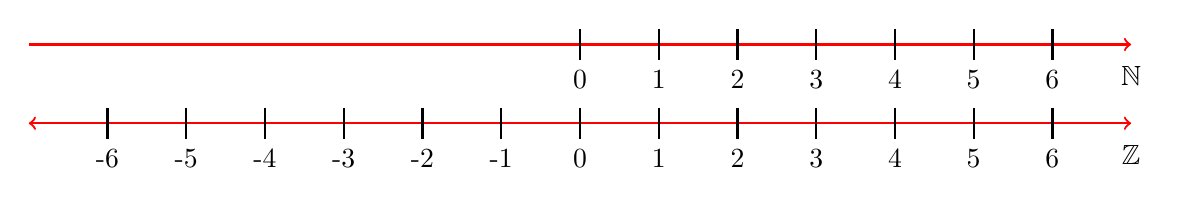
\begin{tikzpicture}
			\draw[thick, red, ->] (0,0) -- (14,0);
			\draw[thick] (7,.2) -- (7,-.2) node[anchor=north] {0};
			\draw[thick] (8,.2) -- (8,-.2) node[anchor=north] {1};
			\draw[thick] (9,.2) -- (9,-.2) node[anchor=north] {2};
			\draw[thick] (10,.2) -- (10,-.2) node[anchor=north] {3};
			\draw[thick] (11,.2) -- (11,-.2) node[anchor=north] {4};
			\draw[thick] (12,.2) -- (12,-.2) node[anchor=north] {5};
			\draw[thick] (13,.2) -- (13,-.2) node[anchor=north] {6};
			\draw (14,-.4) node {$ \N $};
			\draw[thick, red, <->] (0,-1) -- (14,-1);
			\draw[thick] (1,-.8) -- (1,-1.2) node[anchor=north] {-6};
			\draw[thick] (2,-.8) -- (2,-1.2) node[anchor=north] {-5};
			\draw[thick] (3,-.8) -- (3,-1.2) node[anchor=north] {-4};
			\draw[thick] (4,-.8) -- (4,-1.2) node[anchor=north] {-3};
			\draw[thick] (5,-.8) -- (5,-1.2) node[anchor=north] {-2};
			\draw[thick] (6,-.8) -- (6,-1.2) node[anchor=north] {-1};
			\draw[thick] (7,-.8) -- (7,-1.2) node[anchor=north] {0};
			\draw[thick] (8,-.8) -- (8,-1.2) node[anchor=north] {1};
			\draw[thick] (9,-.8) -- (9,-1.2) node[anchor=north] {2};
			\draw[thick] (10,-.8) -- (10,-1.2) node[anchor=north] {3};
			\draw[thick] (11,-.8) -- (11,-1.2) node[anchor=north] {4};
			\draw[thick] (12,-.8) -- (12,-1.2) node[anchor=north] {5};
			\draw[thick] (13,-.8) -- (13,-1.2) node[anchor=north] {6};
			\draw (14,-1.4) node {$ \Z $};
		\end{tikzpicture}
		\caption{The natural numbers and integers ordered number lines.}
	\end{figure}
	Clearly the natural numbers and integers are not ``comprehensive'' in that they have many gaps. This is what led us to define the rational numbers $ \Q $. It isn't immediate just how well the rationals do at covering the holes in the integers. We can get a sense of this by introducing a property of the rationals. 
	\begin{proposition}{(Interspersing of integers by rationals)}
		For any $ x,y\in\Q $ where $ x<y $, there exists a third rational number $ z\in\Q $ such that $ x<z<y $.
	\end{proposition}
	\begin{proof}
		Let there be two rationals $ x,y\in\Q $ such that $ x<y $. We can define the third rational number of interest as $ z=(x+y)/2 $. We can show that $ x<z<y $ by using arithmetic.
		\begin{align*}
			x&<y\\\frac{x}{2}&<\frac{y}{2}\\\frac{x}{2}+\frac{y}{2}&<\frac{y}{2}+\frac{y}{2}\\z&<y
		\end{align*} 
		And we can arrive at $ x<z $ by adding $ x/2 $ to each side of the given inequality.
		\begin{align*}
			x&<y\\\frac{x}{2}&<\frac{y}{2}\\\frac{x}{2}+\frac{x}{2}&<\frac{y}{2}+\frac{x}{2}\\x&<z
		\end{align*} 
	\end{proof}
	\begin{example}
		
		Take the rational numbers $ 0 $ and $ 1 $. Using the construction given in the previous proof we have $$ \frac{0+1}{2}=\frac{1}{2}$$ is between 0 and 1. We can now repeat this process using the pairs $ (0,1/2) $ and $ (1/2,1) $. \begin{align*}
			\frac{0+1/2}{2}=\frac{1}{4}\\\frac{1/2+1}{2}=\frac{3}{4}
		\end{align*}
		We could repeat this process an infinite number of times, in effect ``filling in'' gaps in $ \Z $ by successively taking the average of two rational numbers. Figure 2 shows this process on the unit interval in the rationals. 
		\begin{figure}[h]
			\centering
			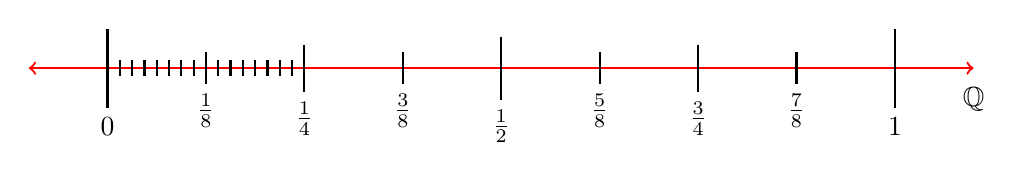
\begin{tikzpicture}
				\draw[thick, red, <->] (-1,0) -- (11,0);
				\draw[thick] (0,.5) -- (0,-.5) node[anchor=north] {0};
				\draw[thick] (5,.4) -- (5,-.4) node[anchor=north] {$ \frac{1}{2} $};
				\draw[thick] (2.5,.3) -- (2.5,-.3) node[anchor=north] {$ \frac{1}{4} $};
				\draw[thick] (7.5,.3) -- (7.5,-.3) node[anchor=north] {$ \frac{3}{4} $};
				\draw[thick] (8.75,.2) -- (8.75,-.2) node[anchor=north] {$ \frac{7}{8} $};
				\draw[thick] (1.25,.2) -- (1.25,-.2) node[anchor=north] {$ \frac{1}{8} $};
				\draw[thick] (6.25,.2) -- (6.25,-.2) node[anchor=north] {$ \frac{5}{8} $};
				\draw[thick] (3.75,.2) -- (3.75,-.2) node[anchor=north] {$ \frac{3}{8} $};
				\draw[thick] (10,.5) -- (10,-.5) node[anchor=north] {1};
				\draw[thick] (0.15625,.1) -- (0.15625,-.1);
				\draw[thick] (0.3125,.1) -- (0.3125,-.1);
				\draw[thick] (0.625,.1) -- (0.625,-.1);
				\draw[thick] (0.46875,.1) -- (0.46875,-.1);
				\draw[thick] (0.78125,.1) -- (0.78125,-.1);
				\draw[thick] (0.9375,.1) -- (0.9375,-.1);
				\draw[thick] (1.09375,.1) -- (1.09375,-.1);
				\draw[thick] (1.40625,.1) -- (1.40625,-.1);
				\draw[thick] (1.5625,.1) -- (1.5625,-.1);
				\draw[thick] (1.71875,.1) -- (1.71875,-.1);
				\draw[thick] (1.875,.1) -- (1.875,-.1);
				\draw[thick] (2.03125,.1) -- (2.03125,-.1);
				\draw[thick] (2.1875,.1) -- (2.1875,-.1);
				\draw[thick] (2.34375,.1) -- (2.34375,-.1);
				\draw (11,-.4) node {$ \Q $};
				
			\end{tikzpicture}
			\caption{}
		\end{figure}\\
		The key question is whether or not this fills \textit{all} the gaps in the integers.
	\end{example}
	While , and more formally , may lead us to believe that the rational numbers have no gaps, this is unfortunately not the case. There are two classic examples that arise from two of the most basic geometric constructions. 
	\begin{example}
		Suppose we have a circle with diameter $ d $ and circumference $ c $. In this case, the ratio give by $ c/d $ is not an element of the rational numbers. This familiar ratio is written as $ \pi $. For the moment, we can take this as fact. We have not yet developed the tools required to proof that $ \pi\notin\Q $, but we will return to this.  
	\end{example}
	\begin{example}
		Suppose there is an isosceles right triangle with legs of length 1, as shown in Figure 3. We want to find the length of the hypotenuse $ x $. 
		\begin{figure}[h]
			\centering
			\begin{tikzpicture}
				\draw[thick] (0,0) -- (8,0);
				\draw[thick] (0,0) -- (0,8);
				\draw[thick] (8,0)--(0,8);
				\draw[thick] (0,0) rectangle (.5,.5);
				\draw[thick] (4,.2)--(4,-.2)node[anchor=north]{1};
				\draw[thick] (.2,4)--(-.2,4)node[anchor=east] {1};
				\draw (4.3,4.3) node {$ x $};
			\end{tikzpicture}
			\caption{}
		\end{figure}\\
		This is a simple application of the Pythagorean Theorem. \begin{align*}
			1^2+1^2&=x^2\\2&=x^2
		\end{align*}
		But this equation has no rational solution, something we can formally prove. 
	\end{example}
	\begin{proposition}
		There exists no rational number $ x $ which satisfies $ x^2=2 $. 
	\end{proposition}
	\begin{proof}
		For the sake of contradiction, suppose that there exists a rational $ x $ which satisfies $ x^2=2 $. If this were the case, we could write $ x=m/n $ for some $ m,n\in\Z $, where $ m $ and $ n $ are not both even.\footnote{Otherwise we could write $ x $ in simpler terms as $ m $ and $ n $ would have a common factor of 2.}
	\end{proof}
	Any $ x $ which does satisfy $ x^2=2 $ would be \textit{irrational}, in that it is not an element of $ \Q $. 
	\begin{definition}\label{def1.4}
		A number is {\color{red}\textit{irrational}} if it is not an element of $ \Q $. 
	\end{definition}
	\noindent There are \textit{many} irrational numbers, each of which is a gap in the rationals (see Figure 4). 
	\begin{figure}[h]
		\centering
		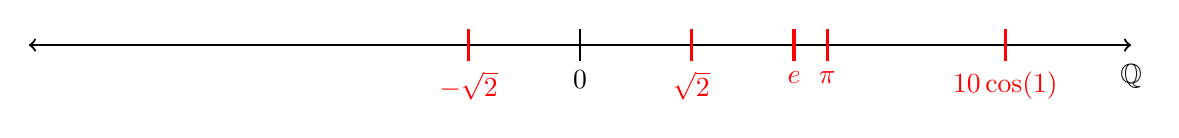
\begin{tikzpicture}
			\draw[thick] (7,.2) -- (7,-.2) node[anchor=north] {0};
			\draw[thick, black, <->] (0,0) -- (14,0);
			\draw (14,-.4) node {$ \Q $};
			\draw[very thick, red ] (10.1415,.2) -- (10.1415,-.2) node[anchor=north] {\color{red}$ \pi $};
			\draw[very thick, red ] (8.4142,.2) -- (8.4142,-.2) node[anchor=north] {\color{red}$ \sqrt{2} $};
			\draw[very thick, red ] (5.5858,.2) -- (5.5858,-.2) node[anchor=north] {\color{red}$ -\sqrt{2} $};
			\draw[very thick, red ] (9.7182,.2) -- (9.7182,-.2) node[anchor=north] {\color{red}$ e $};
			\draw[very thick, red ] (12.403,.2) -- (12.403,-.2) node[anchor=north] {\color{red}$ 10\cos(1) $};
		\end{tikzpicture}
		\caption{}
	\end{figure}\\
	Our goal now becomes defining a set of numbers that includes not only the rationals, but also all of the irrationals. We began with the natural numbers, and then defined a set $ \Z $ which included the additive inverses of the natural numbers. Then we filled more of the gaps in the integers by taking the ratios of integers. We are now faced with the task of defining a set which eliminates the gaps caused by irrational numbers, and doing so eniterly with the set $ \Q $. 
	\subsection{$ \sup $ and $ \inf $}
	Before informally constructing the real numbers, it is worth thinking about why $ \Q $ has these ``holes'', and how it relates to a specific property of sets. It goes without saying that, all the sets of numbers we've discussed up until now have some ordering to them. We can make this formal by defining an ordered set.
	\begin{definition}\label{def1.5}
		An \textit{\color{red}ordered set} is some set $ S $ with a binary relation, denoted by $ < $,\footnote{In this case, ``<'' can mean \textit{any} order. It just so happens that we use the same symbol as the familiar ``less than'' order, because it is the canonical example of such a relation.} which satisfies the following properties:
		\begin{enumerate}
			\item If $ x,y\in S $, then exactly one of the statements $$x<y,\ x=y,\ y<x $$ is true.
			\item If $ x,y,z\in S $, and both $ x<y $ and $ y<z $, then $ x<z $. 
		\end{enumerate}
	\end{definition}  
	The statement $ ``x<y'' $ is read as ``$ x  $ is less than $ y $.''We could also write $ y>x $ instead of $ x<y $. If we were to negative $ y<x $ (``$ y $ is not less than $ x $''), we would arrive at ``y is either greater than $ x $ or equal to $ x $.'' This is denoted as $ y\ge x $. 
	\begin{example}
		The set $ \Q $ is a well ordered set if we define $ < $ in the following way for $ x,y\in\Q $:
		$$ x<y\coloneqq y-x \text{ is a postiive rational number}.   $$ Note that we can only relate objects that belong to $ \Q $. This means that we have no way of comparing rational numbers and the solution to the equation $ x^2=2 $.  
	\end{example}
	We can use the order relation on an ordered set to define bounds on sets.
	\begin{definition}\label{def1.6}
		Suppose $ S $ is an ordered set, and $ E\subseteq S $. If there exists a $ \beta\in S $ such that $ x\le\beta $ for all $ x\in E $, $ E $ is \textit{\color{red}bounded above}, and $ \beta $ is an \textit{\color{red} upper bound} of $ E $. 
	\end{definition}
	\begin{definition}\label{def1.7}
		Suppose $ S $ is an ordered set, and $ E\subseteq S $. If there exists a $ \beta\in S $ such that $ x\ge\beta $ for all $ x\in E $, $ E $ is \textit{\color{red}bounded below}, and $ \beta $ is a \textit{\color{red} lower bound} of $ E $. 
	\end{definition}
	A subtlety in both definitions that is extremely important, is that upper and lower bounds must be elements of the ordered set $ S $. The next example highlights this. 
	\begin{example}
		Take $ \Z $ to be an ordered set with the natural order. Pick the subset $ E=\{-2,-1,2\}\subseteq \Z $. This set has many upper and lower bounds. For upper bounds we have $ 2,3,4,\ldots $. For lower bounds we have $ -2,-3,-4,\ldots
		$. It may be tempting to say that a fraction such as $ 5/2 $ is an upper bound of $ E $, but it is not. This follows from the fact that $ 5/2\notin \Z $, so we have no means of relating it to elements in $ \Z $. In this particular case, there are upper and lower bounds of the set are included in the set. This need not be the case, as the next example shows.  
	\end{example}
	\begin{example}
		Let's look at the ordered set $ \Q $, and subset $ E=\{x\in\Q\mid 0<x<1\}\subseteq \Q $.\footnote{The use of the familiar interval notation of $ (0,1) $ will be properly defined and restricted to the real numbers in the following section.} In this case, each element of $ \{x\in\Q\mid x\le 0\} $ is a lower bound of $ E $, and  each element of $ \{x\in\Q\mid x\ge 1\} $ is an upper bound of $ E $. Even though $ 0,1\notin E $, they are still least and upper bounds of $ E $ respectively. 
	\end{example}
	\begin{remark}
		It is often obvious what exact order we are talking about when referring to an ordered set, like in the case of $ \Q $ and $ \Z $. In these cases, we'll just assume we're using the natural order.  
	\end{remark}
	We now will introduce two definitions that correspond to a special type of upper and lower bound.
	\begin{definition}\label{def1.8}
		Suppose $ S $ is an ordered set, $ E\subseteq S $, and $ E $ is bounded above. We say that $ \alpha $ is a \textit{\color{red}leas- upper-bound} of $ E $ if:
		\begin{enumerate}
			\item $ \alpha $ is an upper bound of $ E $.
			\item If $ \gamma<\alpha $, then $ \gamma $ is not an upper bound of $ E $.
		\end{enumerate}
		Alternatively, we can refer to $ \alpha $ as the \textit{\color{red}supremum} of $ E $, and write $ \alpha=\sup E $
	\end{definition}
	\begin{definition}\label{def1.9}
		Suppose $ S $ is an ordered set, $ E\subseteq S $, and $ E $ is bounded below. We say that $ \alpha $ is a \textit{\color{red}greatest-lower -bound} of $ E $ if:
		\begin{enumerate}
			\item $ \alpha $ is a lower bound of $ E $.
			\item If $ \gamma>\alpha $, then $ \gamma $ is not a lower bound of $ E $.
		\end{enumerate}
		Alternatively, we can refer to $ \alpha $ as the \textit{\color{red}infimum} of $ E $, and write $ \alpha=\inf E $
	\end{definition}
	\begin{remark}
		Both definitions use the definite article \textit{the} before supremum and infimum. This is because they are unique. This is also implied by the use of the superlative \textit{least} and \textit{greatest}. Nevertheless, this is a result of the definition, and can be properly proven. 
	\end{remark}
	
	\begin{example}
		If we return to Example 1.8, where $ E=\{-2,-1,2\}\subseteq\Z $, we have $ \sup E=2 $ and $ \inf E=-2 $. 
	\end{example}
	\begin{example}
		In example 1.9, $ \inf E=0 $ and $ \sup E=1 $.
	\end{example}
	\begin{example}
		Sticking with the set $ \Q$, consider the subset $ E=\{x\in\Q\mid x^2\le 2\}\subseteq \Q $. This set has no supremum, because the number satisfying $ x^2=2 $ is not an element of $ \Q $ (as shown in Proposition 1.2). We will formally prove this fact shortly. 
	\end{example}
	It is no coincidence that a subset of $ \Q $ fails to have a supremum, because of one of the ``holes'' in $ \Q $. The following definition will help us formalize this relationship. 
	\begin{definition}\label{def1.10}
		Let $ S $ be an ordered set. If for all $ E\subseteq S $, where $ E $ is nonempty and bounded from above, $ \sup E $ exists, then $ S $ has the \textit{\color{red}least-upper-bound} property. 
	\end{definition}
	The least-upper-bound property ensures that any nontrivial subset of an ordered set has a supremum in that ordered set. We could define an equivelent property known as the greatest-lower-bound property. The next two propositions serves as nice examples of the least-upper-bound property, or lack there of,  in action.
	\begin{proposition}
		The set $ \Z $ has the least-upper-bound property.
	\end{proposition}
	The idea behind the following proof takes advantage of the fact that $ \Z $ is discrete. For some set $ E\subseteq \Z $, we can always just look at an upper bound of it, and keep subtracting $ 1 $ until the resulting number is in $ E $. Then we will have found our upper bound.
	\begin{proof}
		We will show that an arbitrary nontrivial set $ E\subseteq \Z $ has a supremum. Let $ x\in E $, and $ \beta $ be an upper bound of $ E $. We know that $ \beta\ge x $ for all $ x\in E $ We can show that $ \sup E $ exists via induction on $ \beta-x $ for our arbitrary $ x\in E $. Our base case is when $ \beta-x=0 $. If this holds, then $ \beta\in E $, so $ \beta\in\Z $ and $ \sup E=\beta $. Now suppose that this statement holds when $ \beta-x=k $ for $ k\in\N $ (this is our induction hypothesis). It is either the case that $ \beta\in E $ or $ \beta\notin E $. If $ \beta\in E $, then $ \sup E=\beta $. If $ \beta \notin E $, then let $ \beta'=\beta -1 $. Then $ \beta' $ is an upper bound of $ E $, and $$\beta'-x=\beta-1-x=\beta-x-1=k+1=1=k .$$ By the induction hypothesis, $ \sup E $ exists.   
	\end{proof}
	\begin{proposition}
		The set $ \Q $ does not have the least-upper-bound property.
	\end{proposition}
	To prove this, we will first establish that $ 2 $ is an upper bound of the set defined in Example 1.12, and then show the set has no supremum via contradiction.
	\begin{proof}
		If suffices to find a single subset of $ \Q $ which fails to have a supremum. Let that set be $ E=\{x\in\Q\mid x^2\le 2\} $. 
		\begin{enumerate}
			\item Suppose for contradiction that $ 2 $ is not an upper-bound of $ E $. Then there exists an $ x\in E $ such that $ x>2 $. This would imply that $ x^2>4 $, which contradicts the assumption that $ x \in E $. 
			\item Suppose for contradiction that $ E $ has a supremum, and that $ \sup E=\alpha $ for $ \alpha\in\Q $. Define a new rational number $ y\in \Q $ as 
			\begin{equation}
				y=\alpha-\frac{\alpha^2-2}{x+2}=\frac{2(\alpha+1)}{\alpha+2}.
			\end{equation}
			Squaring this and subtracting $ 2 $ gives 
			\begin{equation}
				y^2-2=\frac{4(\alpha+1)^2}{(\alpha+2)^2}-\frac{2(\alpha+2)^2}{(\alpha+2)^2}=\frac{2(\alpha^2-2)}{(\alpha+2)^2}.
			\end{equation} We can use $ y $ to reach a contradiction in each possible case, those being: $ \alpha^2<2 $, $ \alpha^2=2 $, $ \alpha^2>2 $.
			\begin{enumerate}
				\item Suppose that $ \alpha^2<2 $. This means that $ \alpha^2-2<0 $, so Equation (1) implies that $ y>\alpha $. At the same time, Equation (2) implies that $ y^2-2<0 $, which means $ y^2<2 $. This gives that $ y\in E $, despite the fact that $ \alpha<y $. This contradicts the fact that $ \alpha $ is an upper-bound of $ E $
				\item Suppose $ \alpha^2=2 $. We already know this cannot be the case by Proposition 1.2. 
				\item  Finally, assume that $ \alpha^2>2 $, giving $ \alpha^2-2=0 $. Equation (1)	implies $ y<\alpha $ while Equation (2) implies $ y^2-2>0 $, meaning $ y^2>2 $. This establishes $ y $ as an upper bound for $ E $, but $ y<\alpha $, which contradicts $ \sup E=\alpha $.  
			\end{enumerate}
		\end{enumerate}
	\end{proof}
	The ``holes'' in $ \Q $ are a result of $ \Q $ not having the least-upper-bound property. In order to perform calculus, we need a set that has this property, otherwise things like continuity and differentiation would not work. This property is not sufficient in and of itself though. If that were the case then we would have stopped extending out set of numbers at $ \Z $. We want a set of numbers as ``comprehensive'' as $ \Q $, but with the least-upper-bound property. It turns out, that this (and a whole lot more) is what we will get from the real numbers.  
	\subsection{The Real Numbers}
	We will now construct the real numbers using only $ \Q $. First, we will define the algebraic structure that the real numbers will take on.
	\begin{definition}\label{def1.11}
		A \textit{\color{red}field} is a set $ F $ with two operations, addition and multiplication, which satisfy the following axioms for all $ x,y,z\in F $:
		\begin{enumerate}
			\item Axioms for addition:
			\begin{enumerate}
				\item $ x+y\in F $ (closed under addition)
				\item $ x+y=y+x $ (commutative)
				\item $ (x+y)+z=x+(y+z) $ (associative)
				\item There exists an element $ 0\in F $ such that $ 0+x=x $ (identity element)
				\item There exists an element $ -x\in F $ such that $ x+(-x)=0 $ (inverse element)
			\end{enumerate}
			\item Axioms for multiplication:
			\begin{enumerate}
				\item $ xy\in F $ (closed under multiplication)
				\item $ xy=yx $ (commutative)
				\item $ (xy)z=x(yz) $ (associative)
				\item There exists an element $ 1\in F $ such that $ 1x=x $ (identity element)
				\item If $ x\neq 0 $, there exists an element $ 1/x\in F $ such that $ x(1/x)=1 $ (inverse element)
			\end{enumerate}
			\item The distributive property:
			$$ x(y+z)=xy+xz$$
		\end{enumerate}
	\end{definition}
	The study of fields is its own entire subject in math, and lives within the discipline if abstract algebra. For more details about fields, see \cite{dummit2004abstract}. These axioms can be used to reach several familiar conclusions about arithmetic in fields, and can be found as formal propositions in \cite{rudin1964principles}. A more specific type of field is that which is also an ordered set.
	\begin{definition}\label{def1.12}
		An \textit{\color{red} ordered field} is a field $ F $ such that
		\begin{enumerate}
			\item $ x+y<x+z $ if $ x,y,z\in F $ and $ y<z $,
			\item $ xy>0 $ if $ x,y\in F $, $ x>0 $, and $ y>0 $. 
		\end{enumerate}
	\end{definition}
	\begin{example}
		The set $ \Q $ is an ordered field. 
	\end{example}
	
	Our goal is now to construct an ordered field which not only contains $ \Q $, but also has the least-upper-bound property. In order to do this we'll use the fact that $ \Q $ has ``holes'' in it. We'll form a pair of set $ (A,B) $ that partition $ \Q $ such that each of these partitions corresponds to a real number. 
	
	\begin{definition}\label{def1.13}
		A \textit{\color{red}Dedekind cut} $ x=(A,B) $ is a pair of subsets $ A,B\subseteq \Q $ satisfying the following:
		\begin{enumerate}
			\item $ A\cup B=\Q $, $ A\cap B=\emptyset $, $ A\neq\emptyset $, and $ B\neq\emptyset $.
			\item If $ a\in A $ and $ b\in B $, then $ a<b $.
			\item $ A $ contains no largest element.
		\end{enumerate}
	\end{definition} 
	\begin{example}
		Let $ A=\{y\in \Q \mid y<0\} $ and $ B=\{y\in\Q\mid y\ge 0\} $. Our cut is $ x=(A,B) $, and can be seen in Figure 5.
		\begin{figure}[h]
			\centering
			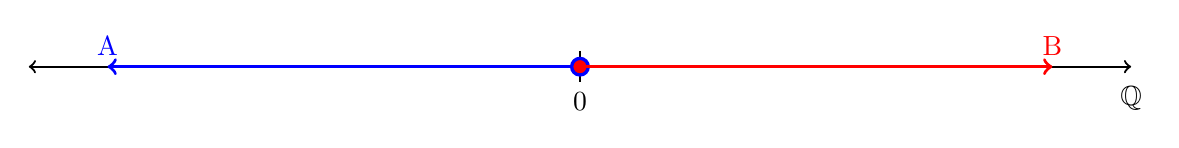
\begin{tikzpicture}
				\draw[thick] (7,.2) -- (7,-.2) node[anchor=north] {0};
				\draw[thick, black, <->] (0,0) -- (14,0);
				\draw (14,-.4) node {$ \Q $};
				\draw[ very thick, blue, ->] (7,0) -- (1,0) node[anchor=south] {A};
				\filldraw[color=blue, fill=red, very thick] (7,0) circle (3pt);
				\draw[ very thick, red, ->] (7,0) -- (13,0) node[anchor=south] {B};
				
			\end{tikzpicture}
			\caption{Dedekind cut corresponding to $ 0\in\Q $.}
		\end{figure}
		This cut uniquely represents $ 0\in\Q $, as no other cut can be defined in this way ``at'' $ 0 $. 
	\end{example}
	\begin{example}
		Perhaps a better example is the cut defined by $ A=\{q\in\Q\mid q\le 0\text{ or }q^2<2 \} $ and $ A=\{q\in\Q\mid q> 0\text{ or }q^2>2 \} $. This cut corresponds to the solution of the equation $ x^2=2 $.  
	\end{example}
	\begin{definition}\label{def1.14}
		A \textit{\color{red}real number} is a Dedekind cut in $ \Q $. The set of real numbers is denoted by $ \R $. 
	\end{definition}
	\begin{definition}\label{def1.15}
		A real number $ x=(A,B) $ is a \textit{\color{red}rational number} if $ B $ contains a smallest element (namely $ x $).
	\end{definition}
	\begin{definition}\label{def1.16}
		A real number $ x=(A,B) $ is a \textit{\color{red}irrational number} if $ B $ contains no smallest element.
	\end{definition}
	\begin{example}
		The cut defined by $ A=\{y\in \Q \mid y<0\} $ and $ B=\{y\in\Q\mid y\ge 0\} $ is rational, as $ B $ has a smallest element in the form of $ 0 $.  
	\end{example}
	\begin{example}
		The cut defined by $A=\{q\in\Q\mid q\le 0\text{ or }q^2<2 \} $ and $ A=\{q\in\Q\mid q> 0\text{ or }q^2>2 \} $ has no smallest element. Therefore it is an irrational number. We will denote this particular number as $ \sqrt{2} $. 
	\end{example}
	Now that we have properly defined $ \R $, we can \textit{finally} refer to the quantity $ \sqrt{2} $! It is no longer a mysterious solution to an equation, and is well defined in $ \R $. This is a relatively small payoff, but the real rewards are the two following theorems. These are the main results of this section, and are of the utmost importance. The first will allow us to perform operations on $ \R $, and the second will play a key role in proving familiar theorems from calculus. The proof of the first result is rather long, and not very informative, so it is omitted. It is important to understand \textit{how} it would be proved though. Before the big reveal, we will define an order on $ \R $
	\begin{definition}\label{def1.17}
		Given real numbers $ x=(A,B) $ and $ y=(C,D) $, we define the following order:$$x\le y\coloneqq A\subseteq C .$$ The inequality is strict if $ A\subseteq C $. 
	\end{definition}
	\begin{example}
		Let $ x=2=(A,B)=(\{y\in \Q \mid y<2\},\{y\in\Q\mid y\ge 2\})$, and $ y=3=(C,D)=(\{z\in \Q \mid z<3\},\{z\in\Q\mid z\ge 3\})$. It should come as no surprise that $ 2<3 $, but this is because $ A\subseteq C $.  
	\end{example}
	\begin{theorem}
		The set $ \R $ is an ordered field containing $ \Q $.
	\end{theorem}
	\begin{proof}
		See the appendix of chapter 1 in \cite{rudin1964principles}. The idea is that addition and multiplication of cuts must be define, and the all the axioms of fields and ordered fields must be verified using the cut definition of a real number. 
	\end{proof}
	\begin{theorem}[Completeness of the real numbers]
		The set $ \R $ has the least-upper-bound property.
		\begin{proof}
			We will show an arbitrary nonempty subset of $ \R $ has a supremum. Let $ E\subseteq \R $, where $ A\neq\emptyset $, have the upper bound $ \beta\in\R $. We may write $ \beta $ as a Dedekind cut, $ \beta=(A,B) $. Additionally, we may express each $ \alpha\in E $ as a cut $ \alpha=(L_\alpha,U_\beta) $. Now we will construct a real number by taking the union of all $ L_\alpha $.
			$$ \gamma=\left(\bigcup_{\alpha\in E}L_\alpha,\Q\backslash \bigcup_{\alpha\in E}L_\alpha\right)=(L,\Q\backslash
			L)=(L,U)$$  
			I claim that $ \sup E=\gamma $.
			
			First we must verify that $ \gamma\in\R $ by showing that $ (L,U) $ is a valid Dedekind cut, and satisfies the requirements of \cref{def1.13}: 
			\begin{enumerate}
				\item The set $ E $ is nonempty, so there exists at least one $ \alpha=(L_\alpha,U_\alpha)\in E $. Because $ L_\alpha\neq\emptyset $ and $ U_\alpha\neq\emptyset $ by definition 1.13, we have $ L\neq\emptyset $ and $ U\neq\emptyset $. By the definition of $ U $ as $ \Q\backslash L $, we have that $  L\cup U=\Q$ and $ L\cap U=\emptyset $. Therefore $ \gamma\in\R $. By construction, $ \alpha\le\gamma $ for all $ \alpha\in E $, making $ \gamma $ an upper bound. 
				\item To show that it is the least-upper-bound, we will now show any number lesser than it cannot be an upper bound. Now suppose $ \delta <\gamma $. This means $  C\subseteq L $, where $ \delta $ is expressed as a cut $ \delta=(C,D) $. This means there exists some $ s\in L $ such that $ s\notin C $. But $ s\in L $, so it is in $ L_\alpha $ for some $ \alpha\in E $. Hence, $ C\subseteq L_\alpha $, giving $ \delta <\alpha $. This shows that $ \delta $ is not an upper bound, meaning $ \sup E =\gamma$.
			\end{enumerate}
		\end{proof}
	\end{theorem}
	
	\begin{example}
		Consider the set of real numbers $ E=\{-1,-1/2,-1/3,-1/4,\ldots\} $. What is the supremum of this set? Intuitively, it should be $ 0 $, but we can verify this by constructing it like we did in the previous proof. Each number in $ E $ corresponds to a cut $ (L_n,U_n) $, for $ L_n=\{x\in\Q\mid x<-1/n\} $ and $ U_n=\{x\in\Q\mid x\ge -1/n\} $, where $ n\in\N $. Our supremum is $$\gamma=\left(\bigcup_{n\in \N}\{x\in\Q\mid x<-1/n\},\Q\backslash \bigcup_{n\in \N}\{x\in\Q\mid x<-1/n\}\right)=(\{x\in\Q\mid x<0\},\{x\in\Q\mid x\ge0\}). $$ Therefore, $ \gamma=0 $.  
	\end{example}
	You will often here the real numbers referred to as ``complete'' because they have the least-upper-bound property. This is because the least-upper-bound property ensures there are no ``gaps'' in the real line like there are in $ \Q $. Theorem 1.2 may be the most important result in real analysis. Remember it well, as it will be used often. Most disciplines in math build on themselves over time, and the fact that $ \R $ has the least-upper-bound property will be our foundation. One could argue it is $ \R $'s defining property.  
	
	Finally, we will adopt the familiar notation of intervals in $ \R $, and add make an important addition to $ \R $. 
	\begin{definition}\label{def1.18}
		We will use the following notation to refer to \textit{\color{red} intervals} of $ \R $:
		\begin{align*}
			(a,b)=\{x\in\R\mid a<x<b\}\\
			[a,b)=\{x\in\R\mid a\le x<b\}\\
			(a,b]=\{x\in\R\mid a<x\le b\}\\
			[a,b]=\{x\in\R\mid a\le x\le b\}
		\end{align*}
		for $ a<b $. 
	\end{definition}
